
\section{Auswertung}
\subsection{Die Hysteresekurve}
Die in Abbildung(\ref{fig:hys}) zu sehende Hysteresekurve ensteht aus den gemessenen Werten,
die im Anhang zu finden sind.

  \begin{figure}
\centering
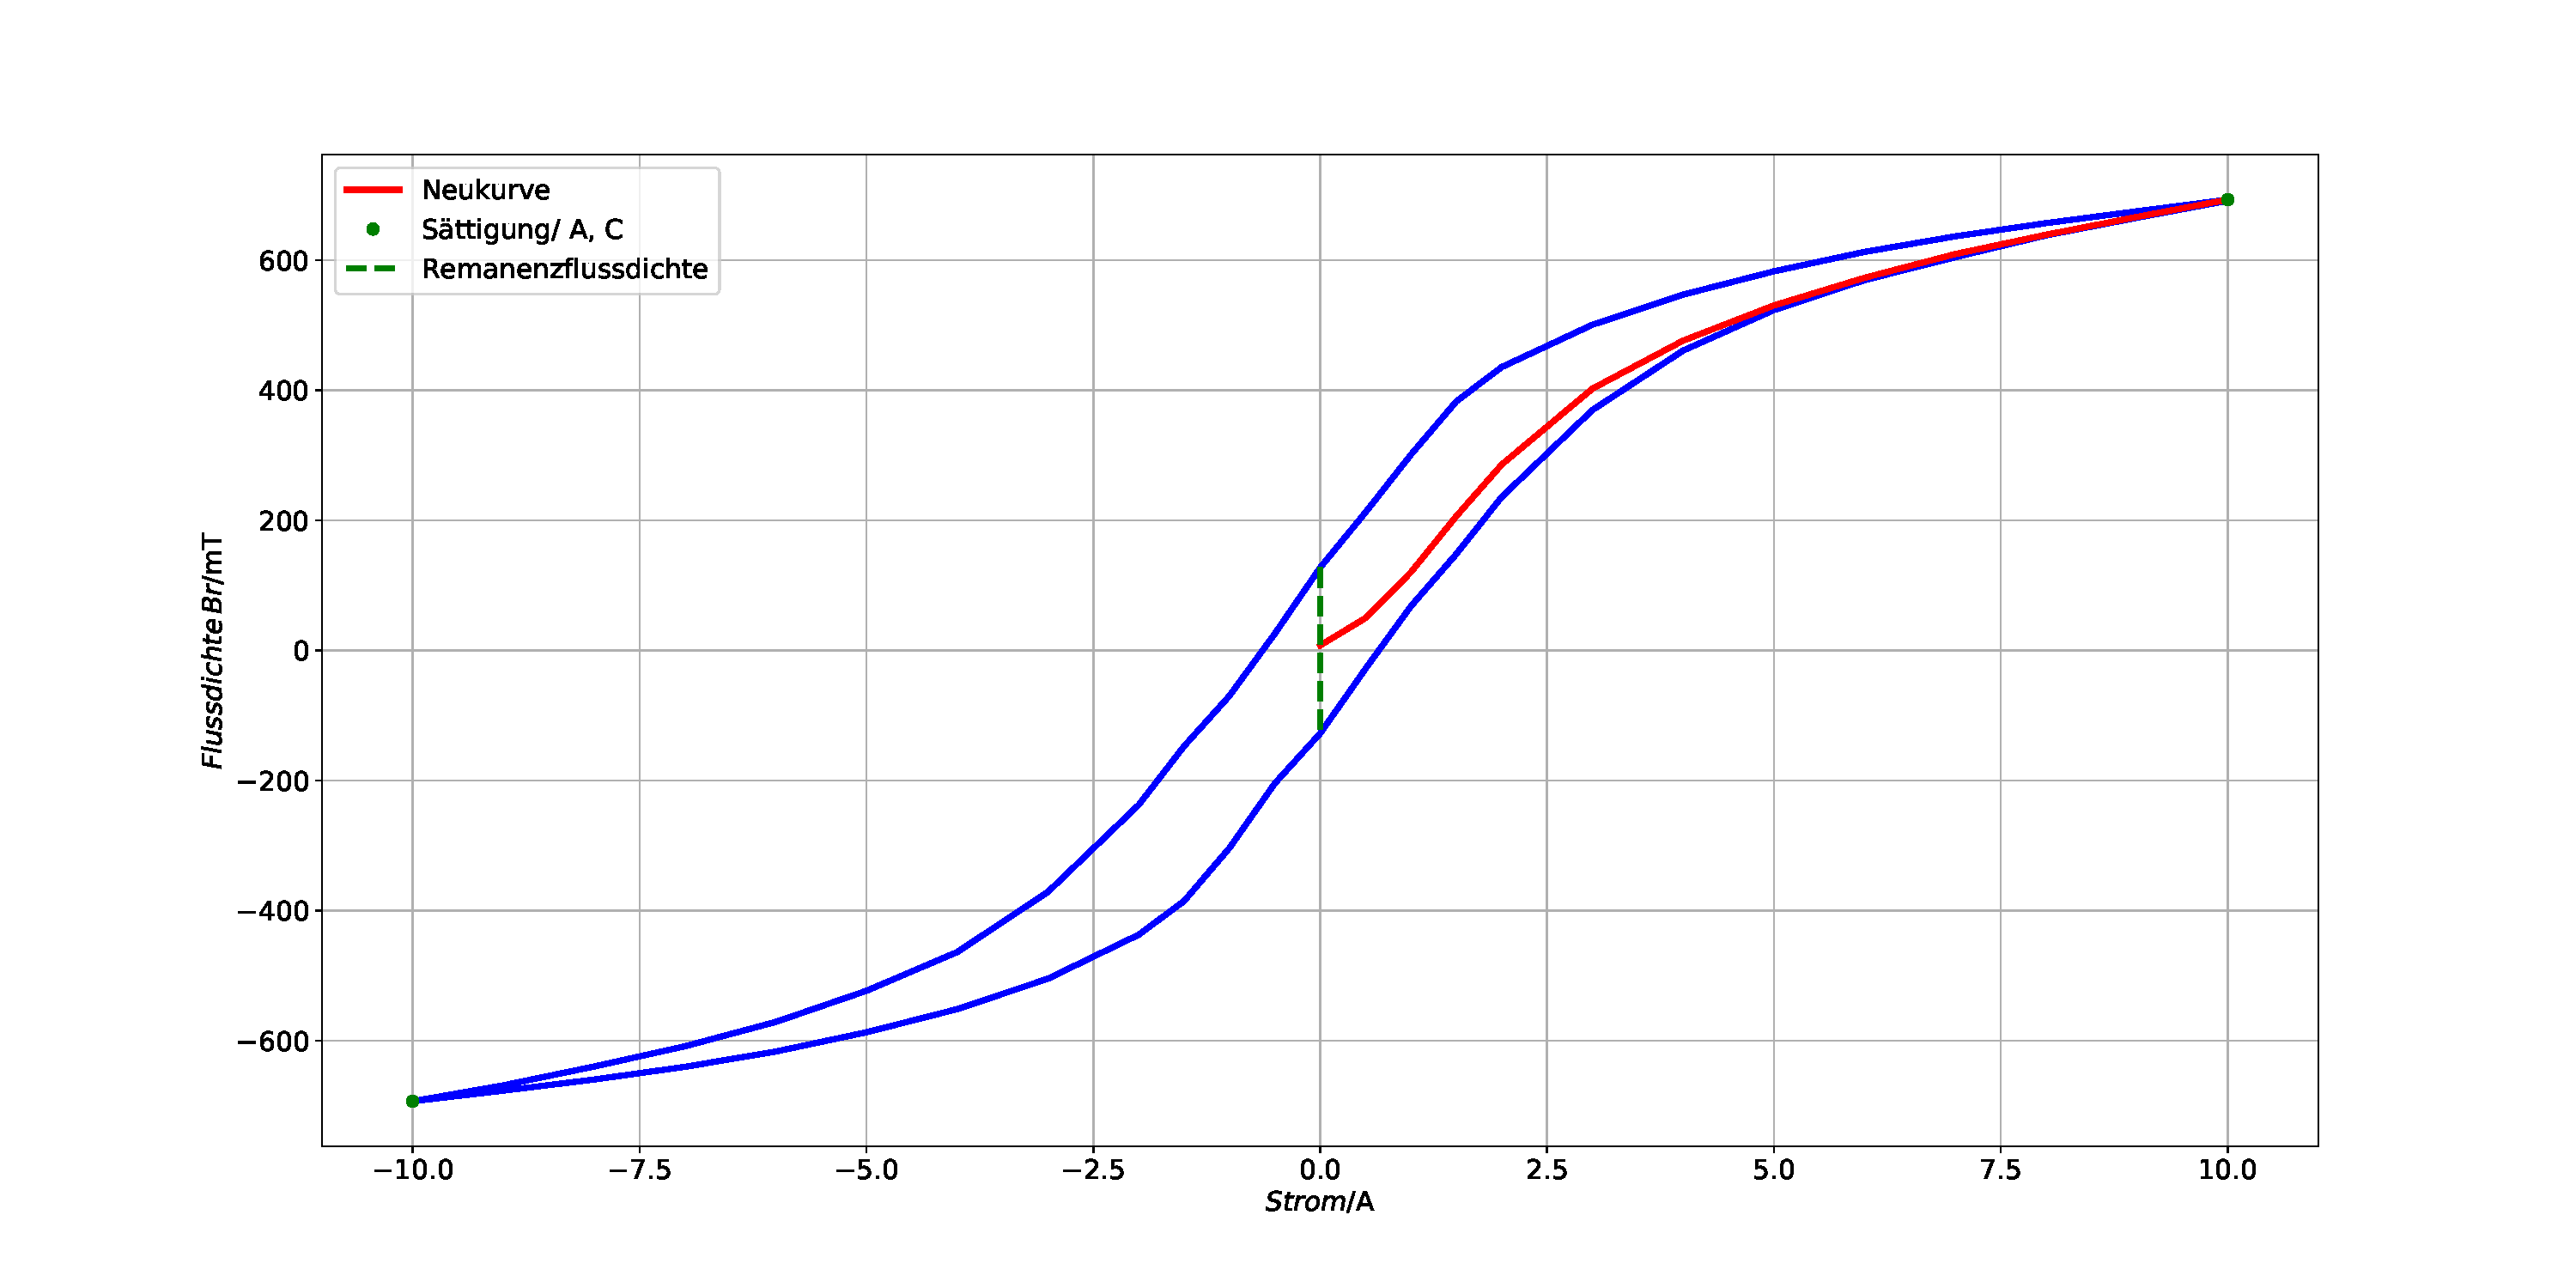
\includegraphics[width=\textwidth]{plothys.pdf}
\caption{Die Hysteresekurve}
\label{fig:hys}
\end{figure}
Die Neukurve führt zu Sättigungspunkt $A$ , der Bei $692\, \mathrm{mT}$ liegt.
Nachdem kompletten Durchlauf liegt der Wert bei $691.3\,\mathrm{mT}$.
Somit folgt:
\begin{equation}
  A = (691,65 \pm 0,00)\, \mathrm{mT}
\end{equation}
Der Sättigungspunkt $C$ wurde nur einmal durchlaufen.
Der Wert liegt bei
\begin{equation}
  C = -693 \,\mathrm{mT}
\end{equation}
 Die Remanenzflussdichte $B_r$ liegt bei
 \begin{align}
   B_{r1} &= 127,4\, \mathrm{mT} & B_{r2} &= -127,5 \, \mathrm{mT}
 \end{align}
 Für die Bestimmung der Koerzitivkraft wurde eine Ausgleichsrechnung mittels Python durchgeführt.
 Die Ausgleichsfunktion lautet:
 \begin{equation}
  f(x) = 693 \cdot tanh(a\cdot(x + b)) + c
 \end{equation}
 Die Parameter für die Funktion von dem Weg von $A$ nach $C$ lautet:
 \begin{align}
 a &= (0,247 \pm 0,006) \\
 b &= (0,74 \pm 0,07)\\
 c &= (-4 \pm 7)
 \end{align}

\begin{figure}
\centering
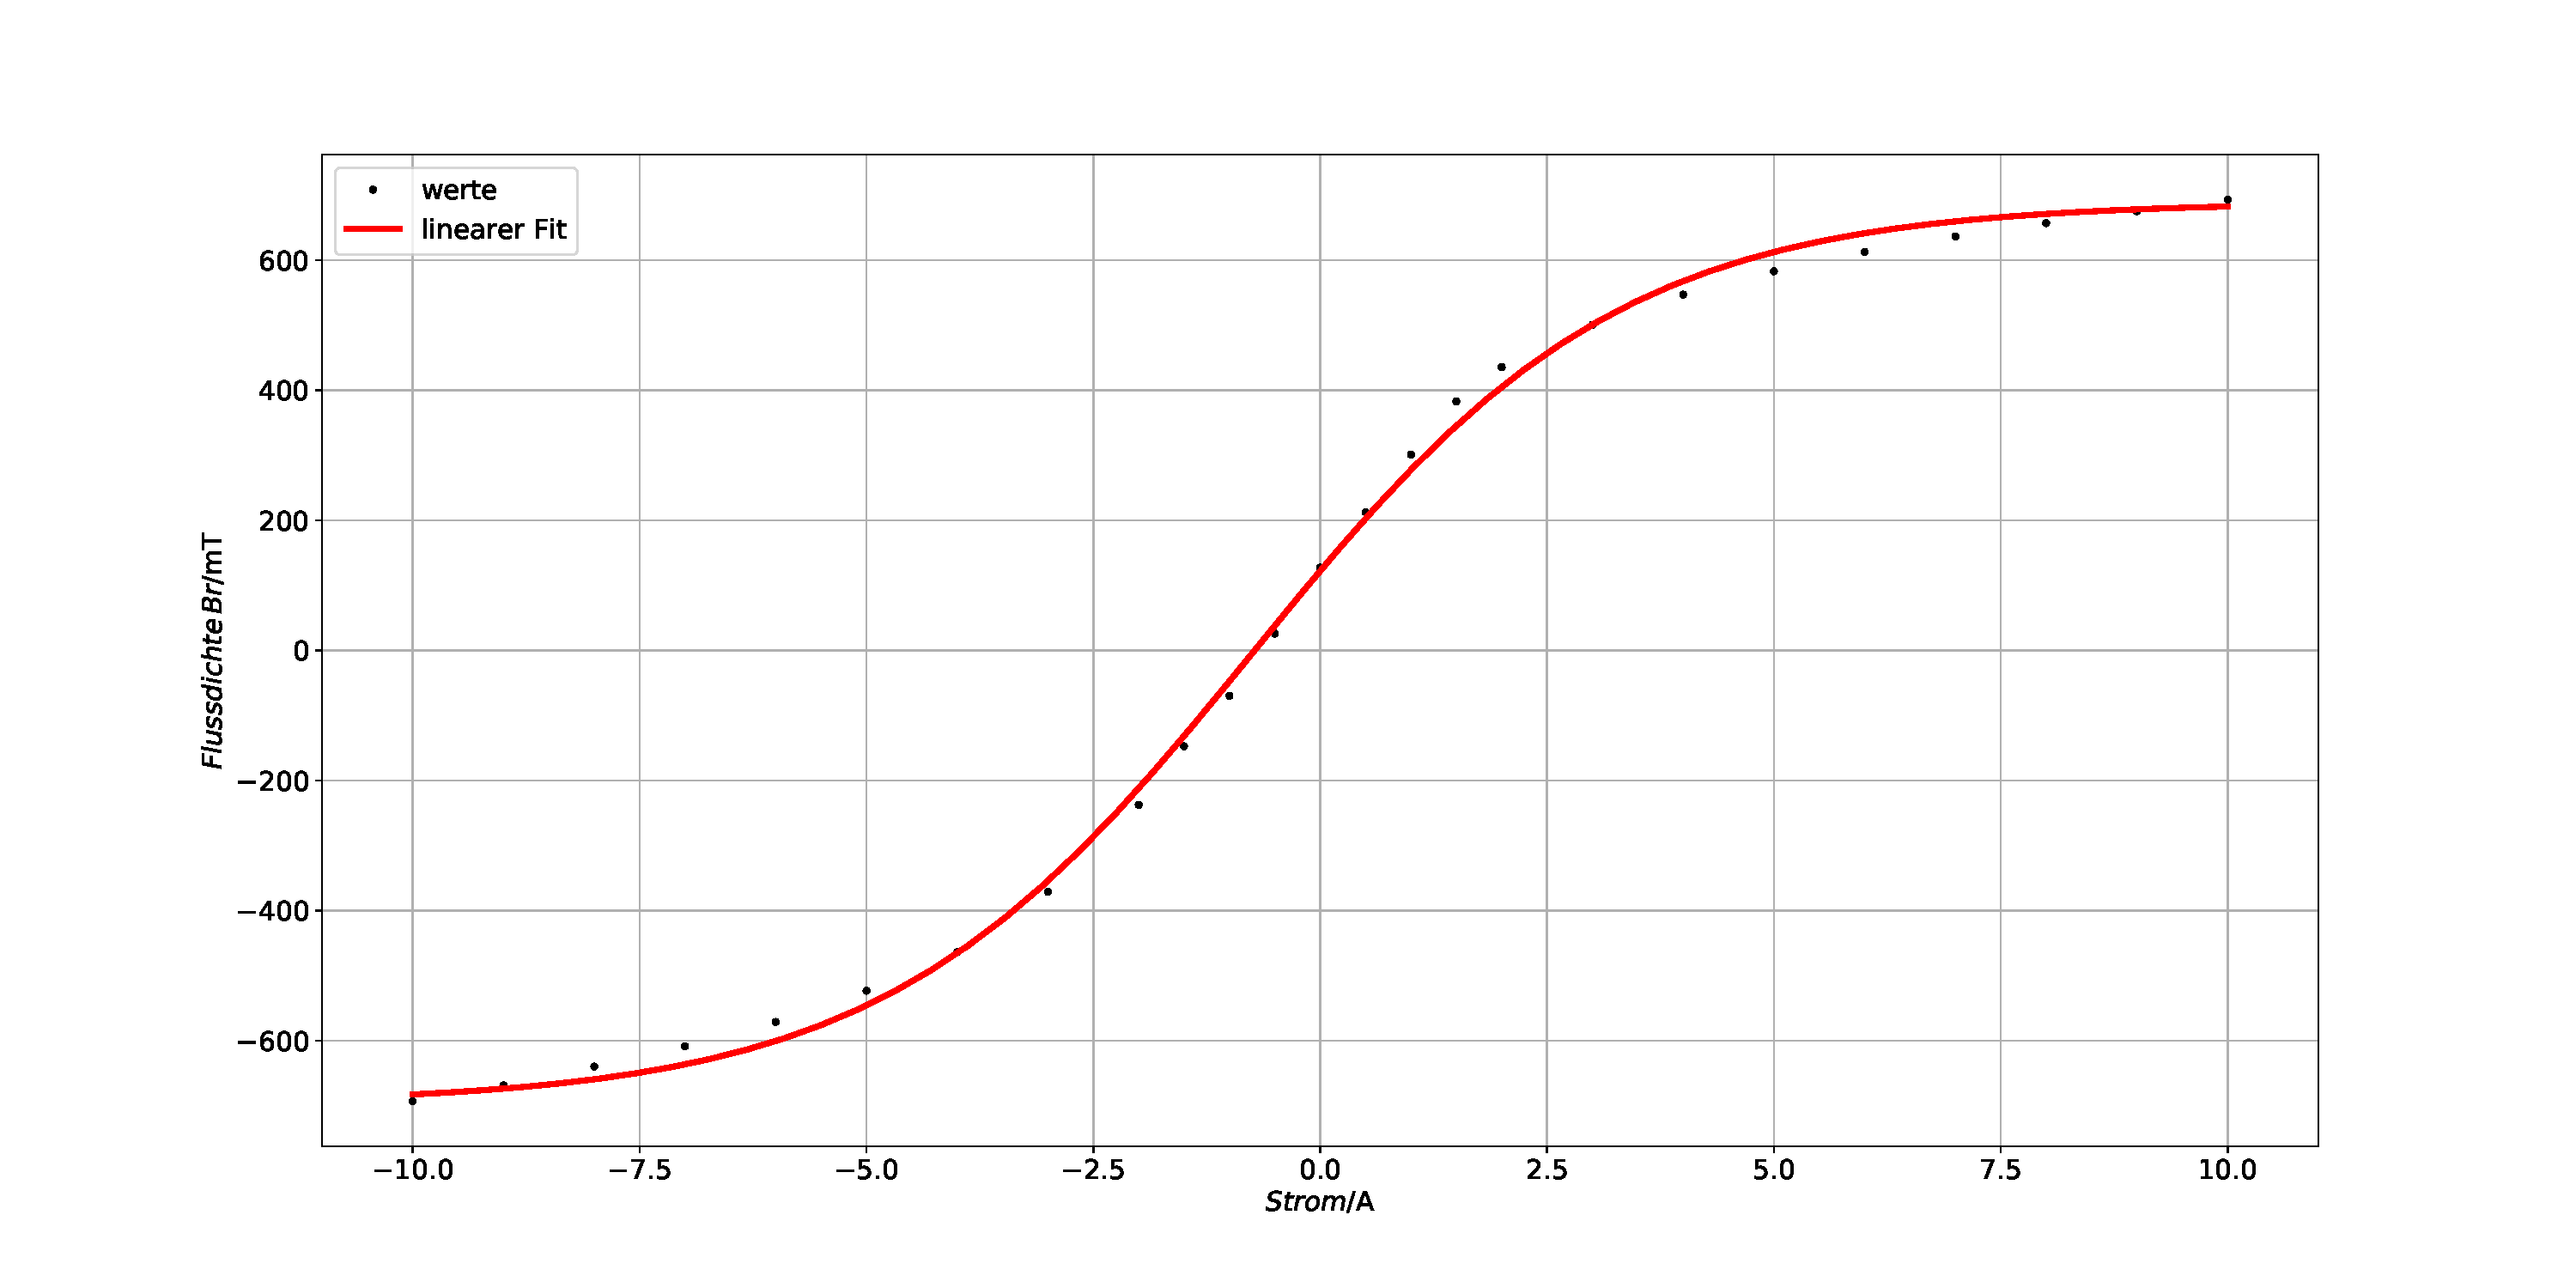
\includegraphics[width=\textwidth]{plotkoertiv.pdf}
\caption{Weg A - C}
\label{fig:koe}
\end{figure}

\begin{figure}
\centering
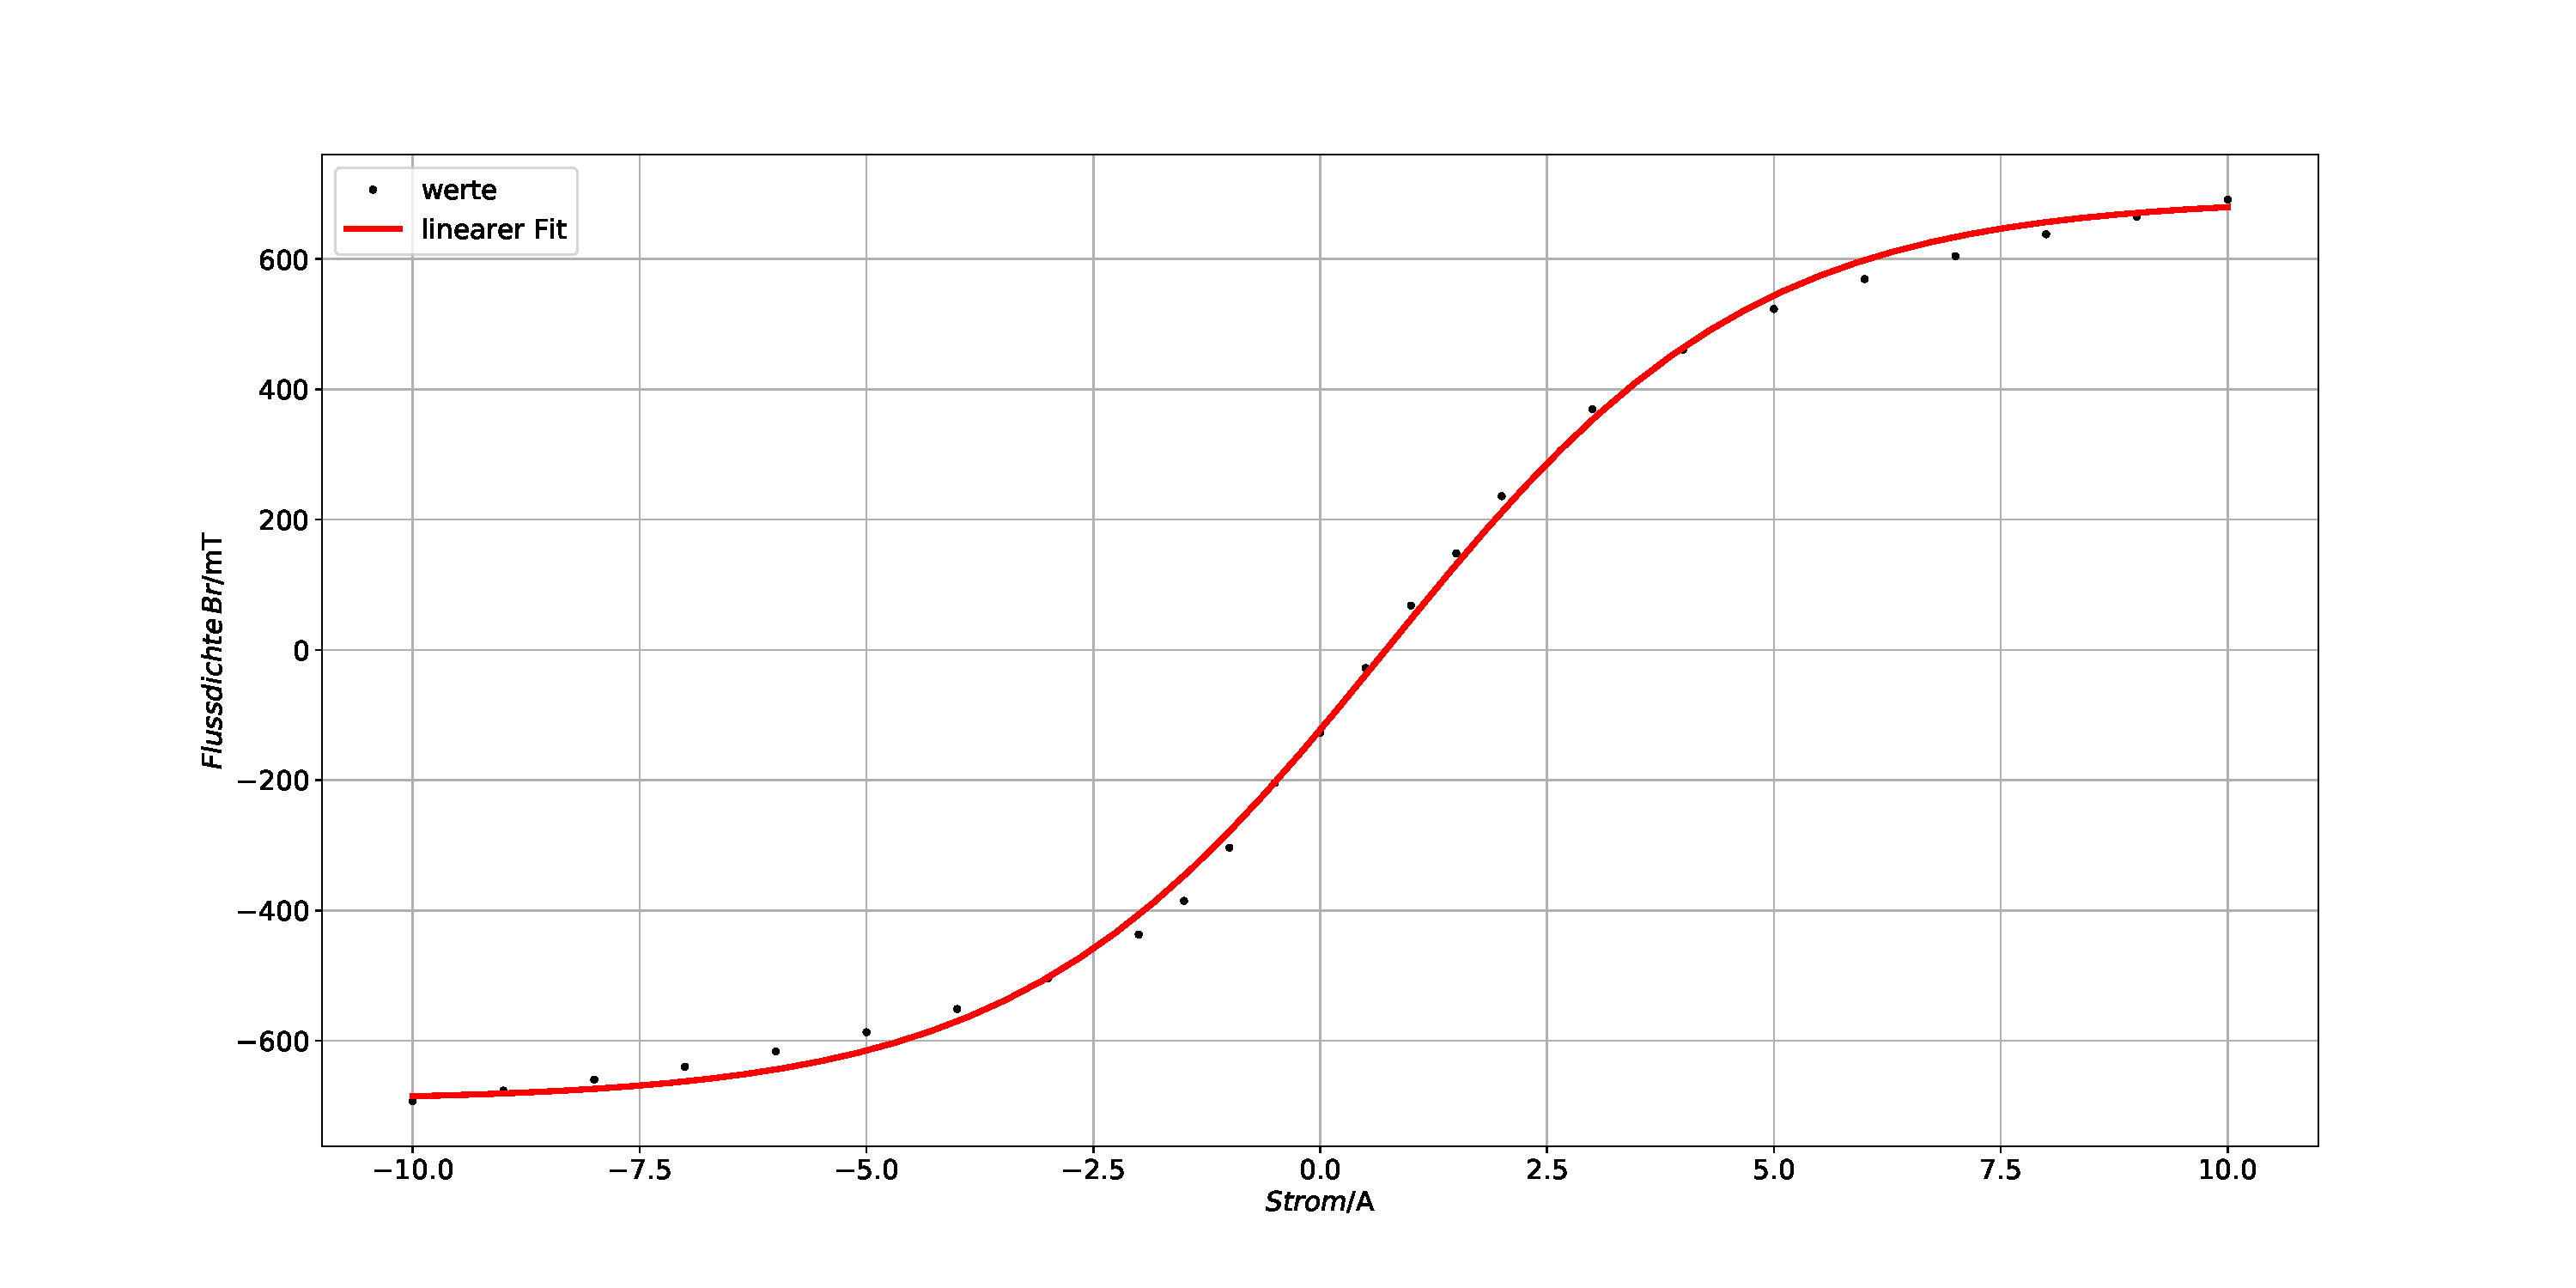
\includegraphics[width=\textwidth]{plotkoertiv2.pdf}
\caption{Weg C - A}
\label{fig:koe2}
\end{figure}
Die Parameter für den Weg von $C$ nach $A$ lauten:
 \begin{align}
   a &= (0,247 \pm 0,005) \,\\
   b &= (-0,73 \pm 0,07)\, \\
   c &= (1 \pm 7)\,
 \end{align}
 Da die $b$ die Verschiebung auf der y-Achse beschreiben, folgt daraus für die Koerzitivkraft $K$:
 \begin{equation}
   K = (73,50 \pm  0,01) \,
\end{equation}
\section{Diskussion}
Die Werte für A und C sollten gleich sein.
Wenn die Funktion zum zweiten mal auf den Sättigungspunkt $A$ trifft, ist dies nicht mehr der Fall.
Je länger gemessen wird, desto fehleranfällig wird die Messung.
